% LuaLaTeX

\documentclass[a4paper, twoside, 12pt]{article}
\usepackage[latin]{babel}
%\usepackage[landscape, left=3cm, right=1.5cm, top=2cm, bottom=1cm]{geometry} % okraje stranky
%\usepackage[landscape, a4paper, mag=1166, truedimen, left=2cm, right=1.5cm, top=1.6cm, bottom=0.95cm]{geometry} % okraje stranky
\usepackage[landscape, a4paper, mag=1400, truedimen, left=0.5cm, right=0.5cm, top=0.5cm, bottom=0.5cm]{geometry} % okraje stranky

\usepackage{fontspec}
\setmainfont[FeatureFile={junicode.fea}, Ligatures={Common, TeX}, RawFeature=+fixi]{Junicode}
%\setmainfont{Junicode}

% shortcut for Junicode without ligatures (for the Czech texts)
\newfontfamily\nlfont[FeatureFile={junicode.fea}, Ligatures={Common, TeX}, RawFeature=+fixi]{Junicode}

\usepackage{multicol}
\usepackage{color}
\usepackage{lettrine}
\usepackage{fancyhdr}

% usual packages loading:
\usepackage{luatextra}
\usepackage{graphicx} % support the \includegraphics command and options
\usepackage{gregoriotex} % for gregorio score inclusion
\usepackage{gregoriosyms}
\usepackage{wrapfig} % figures wrapped by the text
\usepackage{parcolumns}
\usepackage[contents={},opacity=1,scale=1,color=black]{background}
\usepackage{tikzpagenodes}
\usepackage{calc}
\usepackage{longtable}
\usetikzlibrary{calc}

\setlength{\headheight}{14.5pt}

% Commands used to produce a typical "Conventus" booklet

\newenvironment{titulusOfficii}{\begin{center}}{\end{center}}
\newcommand{\dies}[1]{#1

}
\newcommand{\nomenFesti}[1]{\textbf{\Large #1}

}
\newcommand{\celebratio}[1]{#1

}

\newcommand{\hora}[1]{%
\vspace{0.5cm}{\large \textbf{#1}}

\fancyhead[LE]{\thepage\ / #1}
\fancyhead[RO]{#1 / \thepage}
\addcontentsline{toc}{subsection}{#1}
}

% larger unit than a hora
\newcommand{\divisio}[1]{%
\begin{center}
{\Large \textsc{#1}}
\end{center}
\fancyhead[CO,CE]{#1}
\addcontentsline{toc}{section}{#1}
}

% a part of a hora, larger than pars
\newcommand{\subhora}[1]{
\begin{center}
{\large \textit{#1}}
\end{center}
%\fancyhead[CO,CE]{#1}
\addcontentsline{toc}{subsubsection}{#1}
}

% rubricated inline text
\newcommand{\rubricatum}[1]{\textit{#1}}

% standalone rubric
\newcommand{\rubrica}[1]{\vspace{3mm}\rubricatum{#1}}

\newcommand{\notitia}[1]{\textcolor{red}{#1}}

\newcommand{\scriptura}[1]{\hfill \small\textit{#1}}

\newcommand{\translatioCantus}[1]{\vspace{1mm}%
{\noindent\footnotesize \nlfont{#1}}}

% pruznejsi varianta nasledujiciho - umoznuje nastavit sirku sloupce
% s prekladem
\newcommand{\psalmusEtTranslatioB}[3]{
  \vspace{0.5cm}
  \begin{parcolumns}[colwidths={2=#3}, nofirstindent=true]{2}
    \colchunk{
      \input{#1}
    }

    \colchunk{
      \vspace{-0.5cm}
      {\footnotesize \nlfont
        \input{#2}
      }
    }
  \end{parcolumns}
}

\newcommand{\psalmusEtTranslatio}[2]{
  \psalmusEtTranslatioB{#1}{#2}{8.5cm}
}


\newcommand{\canticumMagnificatEtTranslatio}[1]{
  \psalmusEtTranslatioB{#1}{temporalia/extra-adventum-vespers/magnificat-boh.tex}{12cm}
}
\newcommand{\canticumBenedictusEtTranslatio}[1]{
  \psalmusEtTranslatioB{#1}{temporalia/extra-adventum-laudes/benedictus-boh.tex}{10.5cm}
}

% volne misto nad antifonami, kam si zpevaci dokresli neumy
\newcommand{\hicSuntNeumae}{\vspace{0.5cm}}

% prepinani mista mezi notovymi osnovami: pro neumovane a neneumovane zpevy
\newcommand{\cantusCumNeumis}{
  \setgrefactor{17}
  \global\advance\grespaceabovelines by 5mm%
}
\newcommand{\cantusSineNeumas}{
  \setgrefactor{17}
  \global\advance\grespaceabovelines by -5mm%
}

% znaky k umisteni nad inicialu zpevu
\newcommand{\superInitialam}[1]{\gresetfirstlineaboveinitial{\small {\textbf{#1}}}{\small {\textbf{#1}}}}

% pars officii, i.e. "oratio", ...
\newcommand{\pars}[1]{\textbf{#1}}

\newenvironment{psalmus}{
  \setlength{\parindent}{0pt}
  \setlength{\parskip}{5pt}
}{
  \setlength{\parindent}{10pt}
  \setlength{\parskip}{10pt}
}

%%%% Prejmenovat na latinske:
\newcommand{\nadpisZalmu}[1]{
  \hspace{2cm}\textbf{#1}\vspace{2mm}%
  \nopagebreak%

}

% mode, score, translation
\newcommand{\antiphona}[3]{%
\hicSuntNeumae
\superInitialam{#1}
\includescore{#2}

#3
}
 % Often used macros
%%%% Preklady jednotlivych zpevu (nektere se opakuji, a je dobre mit je
% vsechny na jedne hromade)

\newcommand{\trOratioAnteOfficium}{\translatioCantus{Otevři, Pane, má ústa, abych chválil tvé svaté jméno.
Očisti mé srdce od všech marnivých, zvrácených a~jiných myšlenek, osvěť rozum, rozněť cit,
abych mohl důstojně, soustředěně a~zbožně recitovat a~vysloužil si být
vyslyšen před tváří tvé velebnosti. Skrze Krista…}}

\newcommand{\trOratioPostOfficium}{\translatioCantus{\textit{Následující modlitbu
opatřil pro ty, kdo ji zbožně vyřknou po hodinkách, zesnulý papež Lev X.
odpustky za hříchy vzniklé při konání hodinek z~lidské křehkosti. Říká se
vkleče.}
Svatosvaté a~nerozdílné Trojici, ukřižovanému lidství našeho Pána Ježíše
Krista, přeblažené a~přeslavné plodné neporušenosti vždy Panny Marie
i~souhrnu všech svatých buď ode všeho stvoření věčná chvála, čest a~sláva, nám
pak buď dáno odpuštění všech hříchů, po nekonečné věky věků. Amen.}}

% HOURS ---

\newcommand{\trAntI}{\translatioCantus{Jasné narození slavné Panny Marie,
z pokolení (dosl. ze semene) Abrahámova, vzešlé z kmene Judova, z rodu Davidova.}}
\newcommand{\trAntII}{\translatioCantus{Dnes je Narození svaté Panny 
Marie, jejíž předrahý život osvěcuje všechny církve.}}

\newcommand{\trAntIII}{\translatioCantus{Maria, jež vzešla 
z královského rodu, září; myslí i duchem ji zbožně prosíme, aby 
nám pomáhala svými přímluvami.}}

\newcommand{\trAntIV}{\translatioCantus{Srdcem i duchem pějme Kristu 
k slávě o této svaté slavnosti vznešené Rodičky Boží Marie.}}

\newcommand{\trAntV}{\translatioCantus{Příjemně \notitia{?} 
oslavujme Narození blahoslavené Marie,
aby se ona za nás přimlouvala u Pána Ježíše Krista.}}

\newcommand{\trCapituli}{\translatioCantus{Před věky, na počátku mě stvořil, potrvám věčně. Ve svatém Stanu jsem před ním konala službu.}}

\newcommand{\trRespVesp}{\translatioCantus{Buď zdráva, Maria,
plná milosti: \grestar{} Pán s tebou. \Vbardot{} Požehnaná jsi mezi ženami,
a požehnaný plod života (ve smyslu lůna, břicha) tvého.}}

\newcommand{\trVersus}{\translatioCantus{\Vbardot{} Dnes je Narození svaté Panny Marie. \Rbardot{} Jejíž předrahý život osvěcuje všechny církve.}}

\newcommand{\trAntMagnificatI}{\translatioCantus{Konejme památku
veledůstojného narození slavné Panny Marie,
jíž se dostalo mateřské důstojnosti bez ztráty panenské cudnosti.}}

% Tento preklad je vice nez nejisty a ani alternativy, ktere jsem
% videl, me nepresvedcily...
\newcommand{\trAntBenedictus}{\translatioCantus{Slavnostně slavme 
dnešní narození Marie, vždy Panny a Rodičky Boží: v něm se objevuje
vysokost trůnu (totiž Marie, trůnu Božího Syna), aleluja.}}

\newcommand{\trAntMagnificatII}{\translatioCantus{Tvé narození,
Bohorodičko Panno, vyhlásilo radost celému světu:
z tebe totiž vzešlo Slunce spravedlnosti, Kristus, náš Bůh:
jenž zrušil kletbu a dal nám požehnání: přemohl smrt a dal nám život věčný.}}

\newcommand{\trOrationis}{\translatioCantus{Prosíme tě, Bože, 
uděl svým služebníkům dar nebeské milosti,
aby těm, jimž slehnutím blahoslavené Panny vyvstal počátek spásy, 
slavnost k poctě jejího narození přinesla
rozhojnění pokoje.
Skrze tvého Syna, našeho Pána Ježíše Krista, který s tebou žije a kraluje,
Bůh, v jednotě Ducha svatého po všechny věky věků.}}

\newcommand{\trFideliumAnimae}{\translatioCantus{\Vbardot{} Duše věrných ať pro
milosrdenství Boží odpočívají v~pokoji. \Rbardot{} Amen.}}

% Completorium

\newcommand{\trJubeDomne}{\translatioCantus{Rač, pane, požehnat.}}

\newcommand{\trComplBenedictio}{\translatioCantus{Pokojnou noc a~svatou smrt
nechť nám dopřeje všemohoucí Pán. \Rbardot{} Amen.}}

\newcommand{\trComplLectioBr}{\translatioCantus{Buďte střízliví, bděte.
Váš protivník Ďábel obchází jako lev řvoucí a~hledá, koho by pohltil.
Postavte se proti němu pevní ve víře.  Ale ty, Pane, smiluj se nad námi.
\Rbardot{} Bohu díky.}}

\newcommand{\trComplAntI}{\translatioCantus{Rač se smilovati nade mnou,
Hospodine, a vyslyš mou modlitbu.}}

\newcommand{\trComplCapituli}{\translatioCantus{Jsi přece, Hospodine,
uprostřed nás a~jmenujeme se po tobě.  Neopouštěj nás, Pane, náš Bože.}}

\newcommand{\trRespCompl}{\translatioCantus{Do tvých rukou, Pane, \grestar{}
poroučím svého ducha. \Vbardot{} Ty mne zachráníš, Pane, Bože věrný.}}

\newcommand{\trComplVersus}{\translatioCantus{\Vbardot{} Střez mne jako zřítelnici oka,
aleluja. \Rbardot{} Ve stínu svých křídel uschovej mne, aleluja.}}

\newcommand{\trAntSalvaNos}{\translatioCantus{Ochraňuj nás, Pane, když
bdíme, a~buď s~námi, když spíme, ať bdíme s~Kristem a~odpočíváme v~pokoji.}}

\newcommand{\trComplOrationis}{\translatioCantus{Zavítej, prosíme, Pane, sem
do našeho příbytku a~daleko od něj zažeň všechny úklady nepřítele. Ať tu
bydlí tví svatí andělé a~tvoje požehnání buď nad ním stále. Skrze…}}

\newcommand{\trSalveRegina}{\translatioCantus{Zdrávas Královno, matko
milosrdenství, živote, sladkosti a naděje naše, buď zdráva!
K tobě voláme, vyhnaní synové Evy,
k tobě vzdycháme, lkajíce a plačíce
v tomto slzavém údolí.
A proto, orodovnice naše,
obrať k nám své milosrdné oči
a Ježíše, požehnaný plod života svého,
nám po tomto putování ukaž,
ó milostivá, ó přívětivá,
ó přesladká, Panno Maria!}}

\newcommand{\trOraProNobis}{\translatioCantus{\Vbardot{} 
Oroduj za nás, svatá Boží Rodičko,
\Rbardot{} aby nám Kristus dal účast na svých zaslíbeních.}}

% Matutinum

\newcommand{\trMatInvitatorium}{\translatioCantus{}}

\newcommand{\trMatVeniteA}{\translatioCantus{Pojďte, chvalme s~radostí Pána,
s~jásotem slavme Boha, svou spásu; předstupme před tvář jeho s~díky, písně plesu pějme jemu.}}

\newcommand{\trMatVeniteB}{\translatioCantus{Neboť Bůh veliký jest Hospodin, a~král nade všecky bohy.
Jsouť v~jeho ruce všecky hlubiny země, temena hor jsou majetek jeho.}}

\newcommand{\trMatVeniteC}{\translatioCantus{Jehoť jest moře, neb on je učinil; i~souš
je dílo jeho rukou. Pojďme, klanějme se, padněme, klekněme před Pánem, svým
tvůrcem. Jeť on Pán, náš Bůh, a~my jsme lid, jejž on vodí a~ovce, jež pase.}}

\newcommand{\trMatVeniteD}{\translatioCantus{Kéž byste poslechli dnes hlasu jeho:
,,Nezatvrzujte svých srdcí jak v~Hádce, jak v~Pokušení na poušti, kde vaši otcové pokoušeli mne,
zkoušeli mne, ač vídali skutky mé.``}}

\newcommand{\trMatVeniteE}{\translatioCantus{Čtyřicet roků mrzel jsem se na to pokolení
a~řekl jsem: ,,Lid je to myslí stále bloudící``! Oni však nechtěli znáti mé cesty, takže jsem
přisáhl ve svém hněvu: ,,Nedojdou odpočinku mého!\mbox{}``}}

\newcommand{\trMatAntI}{\translatioCantus{}}

\newcommand{\trMatAntII}{\translatioCantus{}}

\newcommand{\trMatAntIII}{\translatioCantus{}}

\newcommand{\trMatVersusI}{\translatioCantus{}}

\newcommand{\trMatAbsolutioI}{\translatioCantus{Vyslyš Pane Ježíši Kriste
prosby svých služebníků \gredagger{} a~smiluj se nad námi, \grestar{} jenž
s~Otcem a~Duchem…}}

\newcommand{\trMatBenedictioI}{\translatioCantus{Rač, pane, požehnat.
Věčný Otec nám stále žehnej. \Rbardot{} Amen.}}

\newcommand{\trMatLecI}{\translatioCantus{Kéž by mě zulíbal polibky svých úst. 
Tvé milování je nad víno lahodnější;
vybraně voní tvé voňavky;
rozlévající se olej je tvé jméno,
proto tě dívky milují.
Strhni mě za sebou, poběžme!
Král mě uvedl do svých komnat;
budeš nám radostí a jásotem.
Víc než víno oslavíme tvé milování;
věru po právu jsi milován!
Snědá jsem, a přece krásná, jeruzalémské dcery,
jako stany kedarské,
jako šalmské závěsy.
}}

\newcommand{\trMatRespI}{\translatioCantus{}}

\newcommand{\trMatBenedictioII}{\translatioCantus{Rač, pane, požehnat.
Jednorozený Boží Syn nám žehnej \grestar{} a nám pomáhej. \Rbardot{} Amen.}}

\newcommand{\trMatLecII}{\translatioCantus{Nehleďte na mou osmahlou pleť:
to mě slunce ožehlo.
Synové mé matky se na mne rozzlobili,
poslali mě hlídat vinice.
A svou vinici, tu jsem nehlídala!
Pověz mi tedy, ty, jehož miluje mé srdce:
kam zavedeš své stádo pást,
kde ho necháš za poledne odpočívat?
Abych už nebloudila jako tulačka
poblíž stád druhů tvých.
Nevíš-li to, nejrásnější z žen,
jdi po stopách stáda
a kůzlata svá zaveď, ať se pasou
poblíž obydlí pastýřů.
Ke své klisně zapřažené do vozu faraonova
tebe, mé milá, přirovnávám.
Stále krásné jsou tvé líce s náušnicemi
i tvé hrdlo v náhrdelnících.}}

\newcommand{\trMatRespII}{\translatioCantus{}}

\newcommand{\trMatBenedictioIII}{\translatioCantus{Rač, pane, požehnat.
Milost Ducha Svatého ať osvítí nám smysly \grestar{} i srdce. \Rbardot{} Amen.}}

\newcommand{\trMatLecIII}{\translatioCantus{Zhotovíme ti zlaté náušnice
a kuličky ze stříbra.
Když král stoluje,
vydechuje můj nard svou vůni.
Můj milý je polštářek s myrhou,
jenž mi odpočívá mezi ňadry.
Můj milý je hrozen šáchoru
ve vinicích v Engadi.
Jak jsi krásná, milá moje,
jak jsi krásná!
Tvé oči jsou holubice.
Jak jsi krásný, můj milý,
jak líbezný!
Naše lože je samá zeleň.
Trámoví našeho domu je z cedru,
naše ostění z cypřiše.}}

\newcommand{\trMatRespIII}{\translatioCantus{}}

\newcommand{\trMatAntIV}{\translatioCantus{}}

\newcommand{\trMatAntV}{\translatioCantus{}}

\newcommand{\trMatAntVI}{\translatioCantus{}}

\newcommand{\trMatVersusII}{\translatioCantus{}}

\newcommand{\trMatAbsolutioII}{\translatioCantus{
Tvá milost a laskavost nechť nám pomáhá, jenž žiješ a vládneš s Otcem a Svatým Duchem na věky věků.}}

\newcommand{\trMatBenedictioIV}{\translatioCantus{Rač, pane, požehnat.
Bůh Otec všemohoucí, \grestar{} buď k nám milostivý a odpouštějící. \Rbardot{} Amen.}}

\newcommand{\trMatLecIV}{\translatioCantus{}}

\newcommand{\trMatRespIV}{\translatioCantus{}}

\newcommand{\trMatBenedictioV}{\translatioCantus{}}

\newcommand{\trMatLecV}{\translatioCantus{}}

\newcommand{\trMatRespV}{\translatioCantus{}}

\newcommand{\trMatBenedictioVI}{\translatioCantus{Rač, pane, požehnat.
Bůh rozněť v nás oheň své lásky. \Rbardot{} Amen.}}

\newcommand{\trMatLecVI}{\translatioCantus{}}

\newcommand{\trMatRespVI}{\translatioCantus{}}

\newcommand{\trMatAntVII}{\translatioCantus{}}

\newcommand{\trMatAntVIII}{\translatioCantus{}}

\newcommand{\trMatAntIX}{\translatioCantus{}}

\newcommand{\trMatVersusIII}{\translatioCantus{}}

\newcommand{\trMatAbsolutioIII}{\translatioCantus{Z okovů našich hříchů,
\grestar{} vysvoboď nás všemohoucí a milosrdný Pán. \Rbardot{} Amen.}}

\newcommand{\trMatBenedictioVII}{\translatioCantus{Rač, pane, požehnat.
Čtení evangelia nechť je nám \grestar{} spásou a ochranou. \Rbardot{} Amen.}}

\newcommand{\trMatLecVIIa}{\translatioCantus{
  Rodokmen Ježíše Krista, syna Davidova, syna Abrahámova:
  Abrahám zplodil Izáka,
  Izák zplodil Jakuba.}}

\newcommand{\trMatLecVIIb}{\translatioCantus{}}

\newcommand{\trMatRespVII}{\translatioCantus{}}

\newcommand{\trMatBenedictioVIII}{\translatioCantus{Rač, pane, požehnat.
\Rbardot{} Amen.}}

\newcommand{\trMatLecVIII}{\translatioCantus{}}

\newcommand{\trMatRespVIII}{\translatioCantus{}}

\newcommand{\trMatBenedictioIX}{\translatioCantus{Rač, pane, požehnat.
Do společnosti občanů nebes \grestar{} ať nás dovede král andělů.
\Rbardot{} Amen.}}

\newcommand{\trMatLecIX}{\translatioCantus{}}

% from the Czech Liturgia horarum
\newcommand{\trTeDeum}{\begin{translatioMulticol}{3}

Bože, tebe chválíme, 
tebe, Pane, velebíme.

Tebe, věčný Otče, 
oslavuje celá země.

Všichni andělé, 
cherubové i~serafové,

všechny mocné nebeské zástupy 
bez ustání volají:

Svatý, Svatý, Svatý, 
Pán, Bůh zástupů.

Plná jsou nebesa i~země 
tvé vznešené slávy.

Oslavuje tě 
sbor tvých apoštolů,

chválí tě 
velký počet proroků,

vydává o~tobě svědectví 
zástup mučedníků;

a~po celém světě 
vyznává tě tvá církev:

neskonale velebný, 
všemohoucí Otče,

úctyhodný Synu Boží, 
pravý a~jediný,

božský Utěšiteli, 
Duchu svatý.

Kriste, Králi slávy, 
tys od věků Syn Boha Otce;

abys člověka vykoupil, 
stal ses člověkem a~narodil ses z~Panny;

zlomil jsi osten smrti 
a~otevřel věřícím nebe;

sedíš po Otcově pravici 
a~máš účast na jeho slávě.

Věříme, že přijdeš soudit, 

a~proto tě prosíme:
přispěj na pomoc svým služebníkům, 
vždyť jsi je vykoupil svou předrahou krví;

dej, ať se radují s~tvými svatými 
ve věčné slávě.

Zachraň, Pane, svůj lid, žehnej svému dědictví, 
veď ho a~stále pozvedej.

Každý den tě budeme velebit 
a~chválit tvé jméno po všechny věky.

Pomáhej nám i~dnes, 
ať se nedostaneme do područí hříchu.

Smiluj se nad námi, Pane, 
smiluj se nad námi.

Ať spočine na nás tvé milosrdenství, 
jak doufáme v~tebe.

Pane, k~tobě se utíkáme, 
ať nejsme zahanbeni na věky. 
\end{translatioMulticol}}

\newcommand{\trMatEvangelium}{\translatioCantus{
  Rodokmen Ježíše Krista, syna Davidova, syna Abrahámova:
  Abrahám zplodil Izáka,
  Izák zplodil Jakuba,
  Jakub zplodil Judu a jeho bratry,
  Juda zplodil Farese a Zaru z Tamary,
  Fares zplodil Esroma,
  Esrom zplodil Arama,
  Aram zplodil Aminadaba,
  Aminadab zplodil Naasona,
  Naason zplodil Salmona,
  Salmon zplodil Boaze z Rahaby,
  Boaz zplodil Jobeda z Rut,
  Jobed zplodil Jessea,
  Jesse zplodil krále Davida.
  David zplodil Šalomouna z Uriášovy ženy,
  Šalomoun zplodil Roboama,
  Roboam zplodil Abiu,
  Abia zplodil Asu,
  Asa zplodil Josafata,
  Josafat zplodil Jorama,
  Joram zplodil Oziáše,
  Oziáš zplodil Joatama,
  Joatam zplodil Achaze,
  Achaz zplodil Ezechiáše,
  Ezechiáš zplodil Manasesa,
  Manases zplodil Amona,
  Amon zplodil Josiáše,
  Josiáš zplodil Jechoniáše a jeho bratry;
  tehdy došlo k odvlečení do Babylonu.
  Po odvlečení do Babylonu:
  Jechoniáš zplodil Salatiela,
  Salatiel zplodil Zorobabela,
  Zorobabel zplodil Abiuda,
  Abiud zplodil Eljakima,
  Eljakim zplodil Azora,
  Ator zplodil Sadoka,
  Sadok zplodil Achima,
  Achim zplodil Eliuda,
  Eliud zplodil Eleazara,
  Eleatar zplodil Matana,
  Matan zplodil Jakuba,
  Jakub zplodil Josefa, manžela Marie,
  z níž se narodil Ježíš, který se nazývá Kristus.}}

\newcommand{\trTeDecetLaus}{\translatioCantus{Tobě chvála, Tobě zpěvy, Tobě
sláva, Bohu Otci i~Synu i~Svatému Duchu, na věky věků. \Rbardot{} Amen.}}

% MASS ---

\newcommand{\trIntroitus}{\translatioCantus{Radujme se všichni
v Pánu, slavíce svátek ke cti Panny Marie: z něj se radují andělé
a spoluchválí Božího Syna. \textit{\color{red}Žl.} Má ústa vydala dobré slovo,
přednáším svá díla králi.}}

\newcommand{\trGraduale}{\translatioCantus{Požehnaná a ctihodná jsi,
Panno Maria: nedotčená (co do panenství) jsi byla shledána matkou
Spasitele. \Vbardot{} Panno Boží Rodičko, ten, jehož nepojme ani celý svět,
se uzavřel do tvých útrob, když se stal člověkem.}}

\newcommand{\trAlleluia}{\translatioCantus{Aleluja. \Vbardot{} Skvělá slavnost
slavné Panny Marie, z pokolení (dosl. ze semene) Abrahámova, vzešlé z kmene 
Judova, z rodu Davidova.}}

\newcommand{\trOffertorium}{\translatioCantus{Blažená jsi, Panno Maria,
tys nosila Stvořitele všeho; porodila jsi toho, který tě utvořil,
a na věky zůstáváš Pannou.}}

\newcommand{\trCommunio}{\translatioCantus{Budou mě blahoslavit
všechna pokolení, protože mi učinil veliké věci ten, který je mocný.}}

% LITTLE HOURS ---

\newcommand{\trVersusTertia}{\translatioCantus{\Vbardot{} \Rbardot{}}}

\newcommand{\trCapituliEtSic}{\translatioCantus{
Tak jsem se usadila na Sionu a v milovaném městě jsem nalezla odpočinek,
v Jeruzalémě vykonávám svou moc.
Zakořenila jsem u lidu plného slývy, na panství Páně, v jeho dědictví.}}

\newcommand{\trVersusSexta}{\translatioCantus{\Vbardot{} \Rbardot{}}}

\newcommand{\trCapituliInPlateis}{\translatioCantus{
Na planině jako skořicovník a akant jsem vydávala vůni, jako vybraná myrha
jsem voněla.}}

\newcommand{\trVersusNona}{\translatioCantus{\Vbardot{} \Rbardot{}}}
 % Czech translations of the proper texts

\newcommand{\annusEditionis}{2020}

%%%% Vicekrat opakovane kousky

\newcommand{\anteOrationem}{
  \rubrica{Ante Orationem, cantatur a Superiore:}

  \pars{Supplicatio Litaniæ.}

  \cuminitiali{}{temporalia/supplicatiolitaniae.gtex}

  \pars{Oratio Dominica.}

  \cuminitiali{}{temporalia/oratiodominica.gtex}

  \rubrica{Deinde dicitur ab Hebdomadario:}

  \cuminitiali{}{temporalia/dominusvobiscum-solemnis.gtex}

  \rubrica{In choro monialium loco Dominus vobiscum dicitur:}

  \sineinitiali{temporalia/domineexaudi.gtex}
}

\setlength{\columnsep}{30pt} % prostor mezi sloupci

%%%%%%%%%%%%%%%%%%%%%%%%%%%%%%%%%%%%%%%%%%%%%%%%%%%%%%%%%%%%%%%%%%%%%%%%%%%%%%%%%%%%%%%%%%%%%%%%%%%%%%%%%%%%%
\begin{document}

% Here we set the space around the initial.
% Please report to http://home.gna.org/gregorio/gregoriotex/details for more details and options
\grechangedim{afterinitialshift}{2.2mm}{scalable}
\grechangedim{beforeinitialshift}{2.2mm}{scalable}
\grechangedim{interwordspacetext}{0.22 cm plus 0.15 cm minus 0.05 cm}{scalable}%
\grechangedim{annotationraise}{-0.2cm}{scalable}

% Here we set the initial font. Change 38 if you want a bigger initial.
% Emit the initials in red.
\grechangestyle{initial}{\color{red}\fontsize{38}{38}\selectfont}

\pagestyle{empty}

%%%% Titulni stranka
\begin{titulusOfficii}
\dies{Die 1. Novembris.}
\nomenFesti{In Festo Omnium Sanctorum.}
\celebratio{Duplex I. classis.}
\end{titulusOfficii}

% graphic
%\vspace{1.5cm}
%\begin{center}
%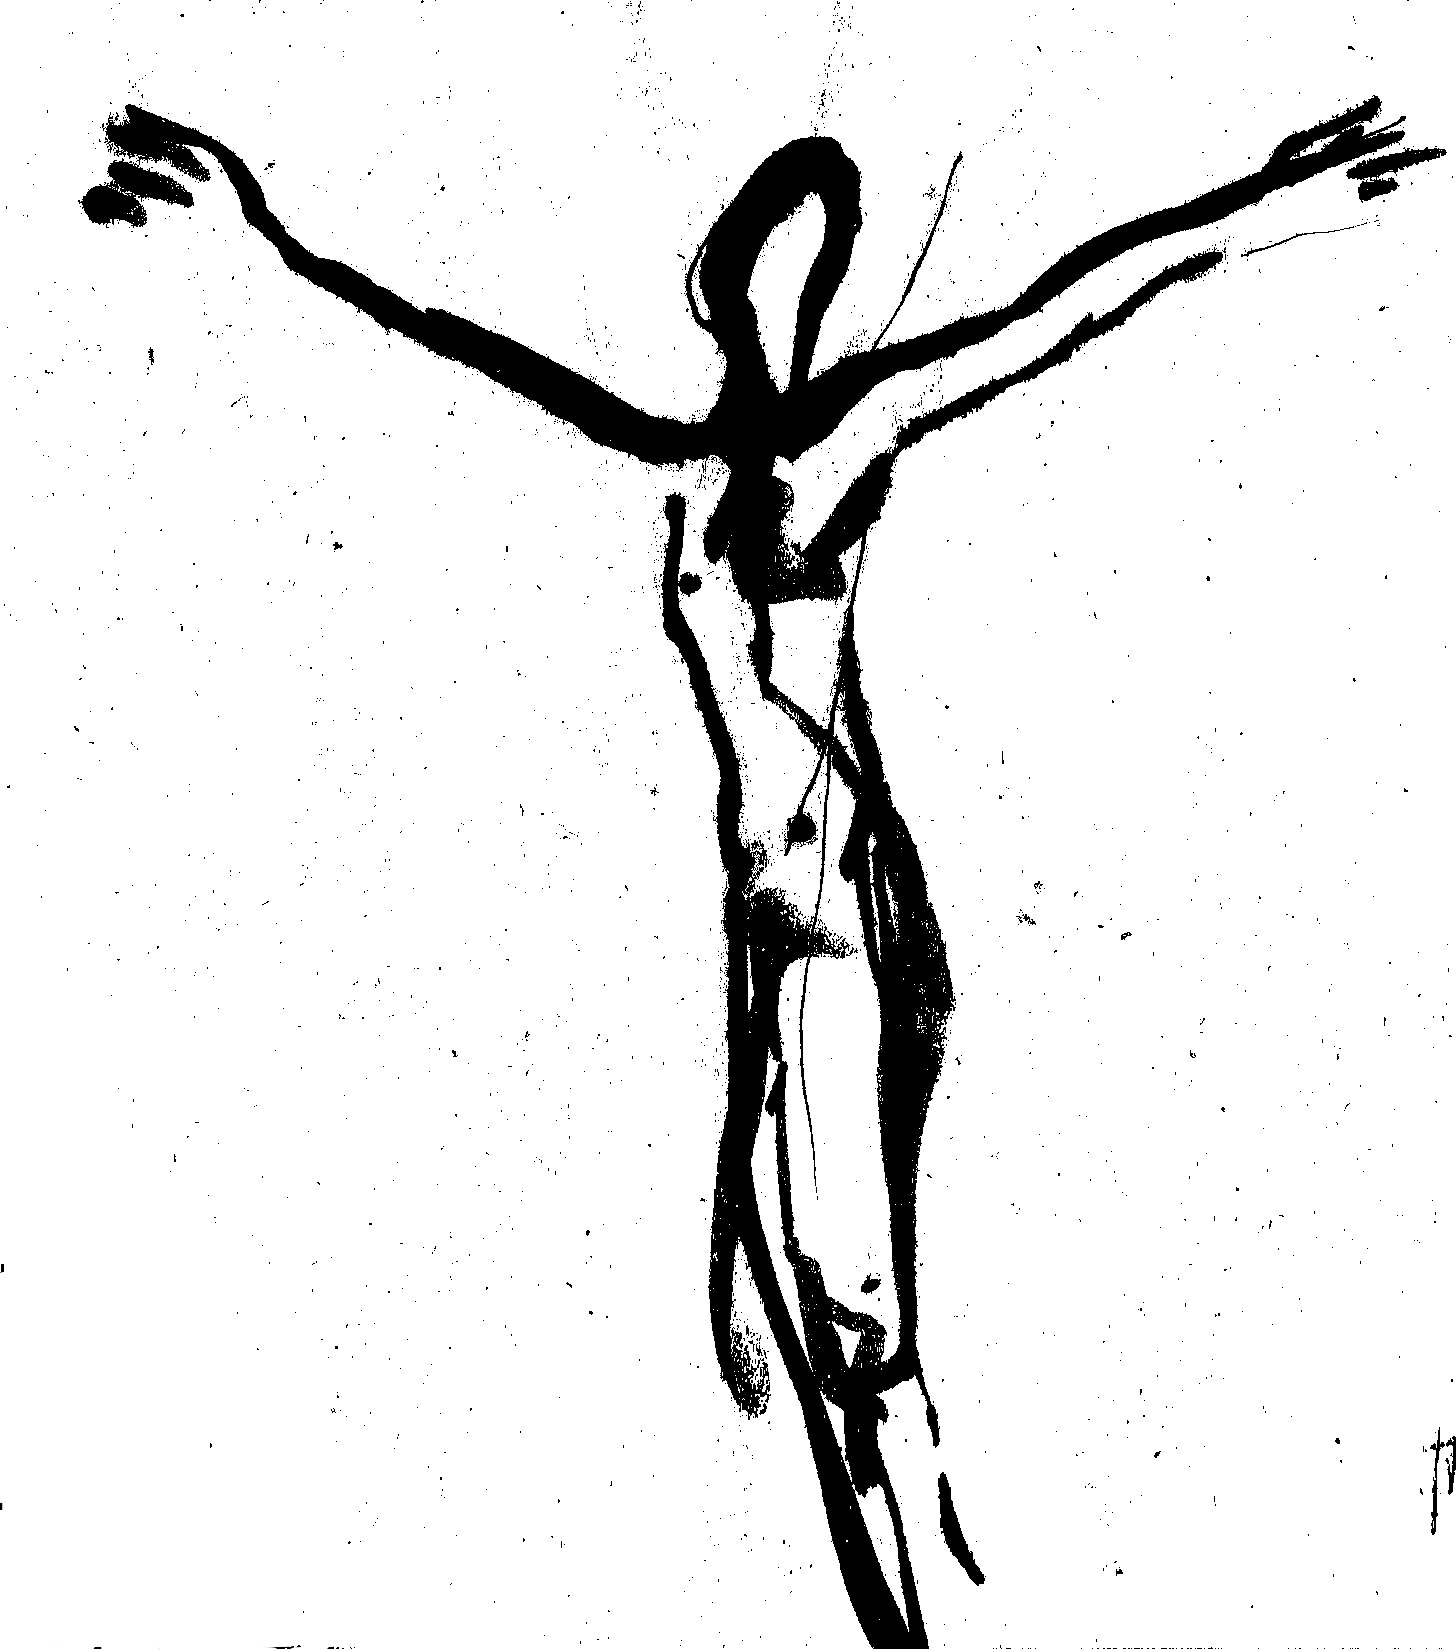
\includegraphics[height=8cm]{crux.jpg}
%\end{center}

\vfill

\begin{center}
%Ad usum et secundum consuetudines chori \guillemotright{}Conventus Choralis\guillemotleft.

%Editio Sancti Wolfgangi \annusEditionis
\end{center}

\pagebreak

\renewcommand{\headrulewidth}{0pt} % no horiz. rule at the header
\fancyhf{}
\pagestyle{fancy}

\cantusSineNeumas

\pars{Oratio ante divinum Officium.}

\lettrine{{\color{red}A}}{peri,} Dómine, os meum ad benedicéndum nomen sanctum tuum:
munda quoque cor meum ab ómnibus vanis, pervérsis, et aliénis
cogitatiónibus:
intelléctum illúmina, afféctum inflámma,
ut digne, atténte ac devóte hoc Offícium recitáre váleam,
et exaudíri mérear ante conspéctum Divínæ Maiestátis tuæ.
Per Christum, Dóminum nostrum.
\Rbardot{} Amen.

Dómine, in unióne illíus divínæ intentiónis,
qua ipse in terris laudes Deo persolvísti,
has tibi Horas \rubricatum{(vel \textnormal{hanc tibi Horam})} persólvo.

%\trOratioAnteOfficium

\vfill

\pars{Oratio post divinum Officium.}

\rubrica{
  Orationem sequentem devote post Officium recitantibus
  Leo Papa X. defectus, et culpas in eo persolvendo ex humana
  fragilitate contractas, indulsit, et dicitur flexis genibus.
}

\lettrine{{\color{red}S}}{acrosánctæ} et indivíduæ Trinitáti,
crucifíxi Dómini nostri Iesu Christi humanitáti,
beatíssimæ et gloriosíssimæ sempérque Vírginis Maríæ
fecúndæ integritáti, 
et ómnium Sanctórum universitáti
sit sempitérna laus, honor, virtus et glória
ab omni creatúra,
nobísque remíssio ómnium peccatórum,
per infiníta sǽcula sæculórum.
\Rbardot{} Amen.

\noindent \Vbardot{} Beáta víscera Maríæ Virginis, quæ portavérunt
ætérni Patris Fílium.\\
\Rbardot{} Et beáta úbera, quæ lactavérunt Christum Dominum.

\rubrica{Et dicitur secreto \textnormal{Pater noster.} et \textnormal{Ave María.}}

%\trOratioPostOfficium

\vfill

\pars{} \scriptura{}

\hora{Ad I. Vesperas.} %%%%%%%%%%%%%%%%%%%%%%%%%%%%%%%%%%%%%%%%%%%%%%%%%%%%%
%\sideThumbs{I. Vesperæ}

\vspace{5mm}
\grechangedim{interwordspacetext}{0.18 cm plus 0.15 cm minus 0.05 cm}{scalable}%
\cuminitiali{}{temporalia/deusinadiutorium-solemnis.gtex}
\grechangedim{interwordspacetext}{0.22 cm plus 0.15 cm minus 0.05 cm}{scalable}%

\vfill
\pagebreak

\pars{Psalmus 1.} \scriptura{Mt. 5, 12; \textbf{H334}}

\vspace{-4mm}

\antiphona{VIII G}{temporalia/ant-gaudeteetexultate.gtex}

%\trAntI

\scriptura{Ps. 112}

\initiumpsalmi{temporalia/ps112-initium-viii-G-auto.gtex}

%\psalmusEtTranslatioT{temporalia/ps112-comb.tex}{10cm}
\input{temporalia/ps112.tex} \Abardot{}

\vfill
\pagebreak

\pars{Psalmus 2.} \scriptura{Cf. 2 Esdr. 2, 35; \textbf{H255}}

\vspace{-4mm}

\antiphona{I g}{temporalia/ant-luxperpetua.gtex}

%\trAntII

\scriptura{Ps. 116}

\initiumpsalmi{temporalia/ps116-initium-i-g-auto.gtex}
%\psalmusEtTranslatioT{temporalia/ps116-comb.tex}{10cm}
\input{temporalia/ps116.tex} \Abardot{}

\vfill
\pagebreak

\pars{Psalmus 3.}

\vspace{-4mm}

\antiphona{I D\textsuperscript{2}}{temporalia/ant-eccevideagnum.gtex}

%\trAntIII

\scriptura{Ps. 145}

\initiumpsalmi{temporalia/ps145-initium-i-D2-auto.gtex}
%\psalmusEtTranslatioT{temporalia/ps145-comb.tex}{10cm}
\input{temporalia/ps145.tex} \Abardot{}

\vfill
\pagebreak

\pars{Psalmus 4.} \scriptura{Ap. 19, 5.6; \textbf{H334}}

\vspace{-4mm}

\antiphona{IV E}{temporalia/ant-laudemdicite.gtex}

%\trAntIV

\vspace{-2mm}

\scriptura{Ps. 146}

\vspace{-2mm}

\initiumpsalmi{temporalia/ps146-initium-iv-E-auto.gtex}
%\psalmusEtTranslatioT{temporalia/ps146-comb.tex}{10cm}
\input{temporalia/ps146.tex} \Abardot{}

\vfill
\pagebreak

\pars{Psalmus 5.} \scriptura{Ap. 14, 3; Ap. 22, 1.3; Is. 44, 23; \textbf{H68}}

\vspace{-4mm}

\antiphona{VII a}{temporalia/ant-cantabantsancti.gtex}

%\trAntIV

\scriptura{Ps. 147}

\initiumpsalmi{temporalia/ps147-initium-vii-a-auto.gtex}
%\psalmusEtTranslatioT{temporalia/ps147-comb.tex}{10cm}
\input{temporalia/ps147.tex} \Abardot{}

\vfill
\pagebreak

% Capitulum. %%%
\pars{Capitulum.} \scriptura{Ap. 7, 2-3}

\cuminitiali{}{temporalia/capitulum-EcceEgo.gtex}

% preklad Jeruz. bible
%\trCapituli

\vfill
\pars{Responsorium.} \scriptura{\Rbardot{} Is. 6, 1 \Vbardot{} ibid., 2; \textbf{H416}}

\vspace{-5mm}

\responsorium{I}{temporalia/resp-vididominumsedentem-cumdox.gtex}{}

%\trRespVesp

\vfill
\pagebreak

% Hymnus. %%%
\pars{Hymnus.} \scriptura{Elisagarus (\olddag{} post 837)}

{
\grechangedim{interwordspacetext}{0.20 cm plus 0.15 cm minus 0.05 cm}{scalable}%
\cuminitiali{VIII}{temporalia/hym-ChristeRedemptor.gtex}
\grechangedim{interwordspacetext}{0.22 cm plus 0.15 cm minus 0.05 cm}{scalable}%
}
%\input{cantus/amon33/hym-ChristeRedemptor-bohtext.tex}

\vfill

\pars{Versus.} \scriptura{Ps. 31, 11}

% Versus. %%%
\sineinitiali{temporalia/versus-laetamini.gtex}
    
\noindent %\trVersus

\vfill
\pagebreak

\pars{Canticum B. Mariæ V.} \scriptura{Cf. Co. 1, 16}

\vspace{-4mm}

\antiphona{I D}{temporalia/ant-angeliarchangeli.gtex}

%\trAntMagnificatI

%\vspace{-3mm}

\scriptura{Lc. 1, 46-55}

%\vspace{-2mm}

\initiumpsalmi{temporalia/magnificat-initium-isoll-D.gtex}

%\vspace{-1.5mm}

%\psalmusEtTranslatioT{temporalia/magnificat-comb.tex}{10.3cm}
\input{temporalia/magnificat.tex}

\vfill

\antiphona{}{temporalia/ant-angeliarchangeli.gtex}

\vfill
\pagebreak

\anteOrationem

\pagebreak

%% Oratio. %%%
\pars{Oratio.}

\cuminitiali{}{temporalia/oratio.gtex}
%\trOrationis

\vfill

\rubrica{Hebdomadarius dicit iterum Dominus vobiscum, vel cantor dicit:}

\vspace{2mm}

\sineinitiali{temporalia/domineexaudi.gtex}

\rubrica{Postea cantatur a cantore:}

\vspace{2mm}

\cuminitiali{II}{temporalia/benedicamus-solemnism-1vesp.gtex}

\vspace{1mm}

\vfill
\pagebreak

\hora{Ad Matutinum.} %%%%%%%%%%%%%%%%%%%%%%%%%%%%%%%%%%%%%%%%%%%%%%%%%%%%%%%%%%
%\sideThumbs{Matutinum}

\vspace{2mm}

\cantusSineNeumas

\cuminitiali{}{temporalia/dominelabiamea.gtex}

\vspace{5mm}

\pars{Invitatorium.} \scriptura{Cantor; \textbf{K183r}}

\vspace{-2mm}

\antiphona{II}{temporalia/inv-regemregum.gtex}

\vfill
\pagebreak

\pars{Hymnus.}

\vspace{-5mm}

\antiphona{I}{temporalia/hym-ChristeCaelorum.gtex}

\vfill
\pagebreak

\subhora{In I. Nocturno}

\pars{Psalmus 1.} \scriptura{Ps. 1, 2.6; \textbf{H331}}

\vspace{-4mm}

\antiphona{VIII G\textsuperscript{3}}{temporalia/ant-novitdominus.gtex}

%\trMatAntI

\scriptura{Psalmus 1.}

\initiumpsalmi{temporalia/ps1-initium-viii-G3.gtex}

%\psalmusEtTranslatioT{temporalia/ps1-comb.tex}{10cm}
\input{temporalia/ps1.tex} \Abardot{}

\vfill
\pagebreak

\pars{Psalmus 2.} \scriptura{Ps. 4, 4; \textbf{H331}}

\vspace{-4mm}

\antiphona{VII c\textsuperscript{2}}{temporalia/ant-mirificavit.gtex}

%\trMatAntII

\scriptura{Psalmus 4.}

\initiumpsalmi{temporalia/ps4-initium-vii-c2-auto.gtex}

%\psalmusEtTranslatioT{temporalia/ps4-comb.tex}{10cm}
\input{temporalia/ps4.tex} \Abardot{}

\vfill
\pagebreak

\pars{Psalmus 3.} \scriptura{Ps. 8, 2; \textbf{H331}}

\vspace{-4mm}

\antiphona{I D\textsuperscript{2}}{temporalia/ant-admirabileest.gtex}

%\trMatAntIII

\scriptura{Psalmus 8.}

\initiumpsalmi{temporalia/ps8-initium-i-D2-auto.gtex}

%\psalmusEtTranslatioT{temporalia/ps8-comb.tex}{10cm}
\input{temporalia/ps8.tex} \Abardot{}

\vfill
\pagebreak

\pars{Versus.} \scriptura{Ps. 31, 11}

\sineinitiali{temporalia/versus-laetamini-communis.gtex}

\vspace{5mm}

\sineinitiali{temporalia/oratiodominica-mat.gtex}

\vspace{5mm}

\pars{Absolutio.}

\cuminitiali{}{temporalia/absolutio-exaudi.gtex}

%\trMatAbsolutioI

\vfill
\pagebreak

\cuminitiali{}{temporalia/benedictio-solemn-benedictione.gtex}

%\trMatBenedictioI

\vspace{7mm}

\pars{Lectio I.} \scriptura{Ap. 4, 2-8}

\noindent De libro Apocalýpsis beáti Ioánnis Apóstoli.

\noindent Et ecce sedes pósita erat in cælo, et supra sedem sedens. Et qui sedébat símilis erat aspéctui lápidis iáspidis, et sardínis: et iris erat in circúitu sedis símilis visióni smarágdinæ. Et in circúitu sedis sedília vigínti quátuor: et super thronos vigínti quátuor senióres sedéntes, circumamícti vestiméntis albis, et in capítibus eórum corónæ áureæ. Et de throno procedébant fúlgura, et voces, et tonítrua: et septem lámpades ardéntes ante thronum, qui sunt septem spíritus Dei. Et in conspéctu sedis tamquam mare vítreum símile crystállo: et in médio sedis, et in circúitu sedis quátuor animália plena óculis ante et retro. Et ánimal primum símile leóni, et secúndum ánimal símile vítulo, et tértium ánimal habens fáciem quasi hóminis, et quartum ánimal símile áquilæ volánti. Et quátuor animália, síngula eórum habébant alas senas: et in circúitu, et intus plena sunt óculis: et réquiem non habébant die ac nocte, dicéntia: Sanctus, Sanctus, Sanctus Dóminus Deus omnípotens, qui erat, et qui est, et qui ventúrus est.

\noindent \Vbardot{} Tu autem, Dómine, miserére nobis.
\noindent \Rbardot{} Deo grátias.

\vfill
\pagebreak

\pars{Responsorium 1.} \scriptura{\textbf{H104}}

\vspace{-5mm}

\responsorium{VII}{temporalia/resp-summaetrinitati-CROCHU.gtex}{}

\vfill
\pagebreak

\cuminitiali{}{temporalia/benedictio-solemn-unigenitus.gtex}

%\trMatBenedictioII

\vspace{7mm}

\pars{Lectio II.} \scriptura{Ap. 5, 1-8}

\noindent Et vidi in déxtera sedéntis supra thronum, librum scriptum intus et foris, signátum sigíllis septem. Et vidi ángelum fortem, prædicántem voce magna: Quis est dignus aperíre librum, et sólvere signácula eius? Et nemo póterat neque in cælo, neque in terra, neque subtus terram aperíre librum, neque respícere illum. Et ego flebam multum, quóniam nemo dignus invéntus est aperíre librum, nec vidére eum. Et unus de senióribus dixit mihi: Ne fléveris: ecce vicit leo de tribu Iuda, radix David, aperíre librum, et sólvere septem signácula eius. Et vidi: et ecce in médio throni et quátuor animálium, et in médio seniórum, Agnum stantem tamquam occísum, habéntem córnua septem, et óculos septem: qui sunt septem spíritus Dei, missi in omnem terram. Et venit: et accépit de déxtera sedéntis in throno librum. Et cum aperuísset librum, quátuor animália, et vigínti quátuor senióres cecidérunt coram Agno, habéntes sínguli cítharas, et phíalas áureas plenas odoramentórum, quæ sunt oratiónes sanctórum:

\noindent \Vbardot{} Tu autem, Dómine, miserére nobis.
\noindent \Rbardot{} Deo grátias.

\vfill
\pagebreak

\pars{Responsorium 2.} \scriptura{\Rbardot{} Cf. Mal. 4, 2 \Vbardot{} S. Augustini sermo 18 de Sanctis; \textbf{H307}}

\vspace{-5mm}

\responsorium{I}{temporalia/resp-felixnamquees-CROCHU.gtex}{}

\vfill
\pagebreak

\cuminitiali{}{temporalia/benedictio-solemn-spiritus.gtex}

%\trMatBenedictioIII

\vspace{7mm}

\pars{Lectio III.} \scriptura{Ap. 5, 9-14}

\noindent Et cantábant cánticum novum, dicéntes: Dignus es, Dómine, accípere librum, et aperíre signácula eius: quóniam occísus es, et redemísti nos Deo in sánguine tuo ex omni tribu, et lingua, et pópulo, et natióne: et fecísti nos Deo nostro regnum, et sacerdótes: et regnábimus super terram. Et vidi, et audívi vocem angelórum multórum in circúitu throni, et animálium, et seniórum: et erat númerus eórum míllia míllium, dicéntium voce magna: Dignus est Agnus, qui occísus est, accípere virtútem, et divinitátem, et sapiéntiam, et fortitúdinem, et honórem, et glóriam, et benedictiónem. Et omnem creatúram, quæ in cælo est, et super terram, et sub terra, et quæ sunt in mari, et quæ in eo: omnes audívi dicéntes: Sedénti in throno, et Agno, benedíctio et honor, et glória, et potéstas in sǽcula sæculórum. Et quátuor animália dicébant: Amen. Et vigínti quátuor senióres cecidérunt in fácies suas: et adoravérunt vivéntem in sǽcula sæculórum.

\noindent \Vbardot{} Tu autem, Dómine, miserére nobis.
\noindent \Rbardot{} Deo grátias.

\vfill
\pagebreak

\pars{Responsorium 3.} \scriptura{Ps. 137, 1-2; \textbf{H314}}

\vspace{-5mm}

\responsorium{VIII}{temporalia/resp-inconspectuangelorum-CROCHU.gtex}{}

\vfill
\pagebreak

\subhora{In II. Nocturno}

\pars{Psalmus 4.} \scriptura{Ps. 14, 1.2; \textbf{H331}}

\vspace{-4mm}

\antiphona{VI F}{temporalia/ant-dominequioperati.gtex}

%\trMatAntIV

\scriptura{Psalmus 14.}

\initiumpsalmi{temporalia/ps14-initium-vi-F-auto.gtex}

%\psalmusEtTranslatioT{temporalia/ps14-comb.tex}{10cm}
\input{temporalia/ps14.tex} \Abardot{}

\vfill
\pagebreak

\pars{Psalmus 5.} \scriptura{Ps. 23, 6; \textbf{H331}}

\vspace{-4mm}

\antiphona{III a}{temporalia/ant-haecestgeneratio.gtex}

%\trMatAntV

\scriptura{Psalmus 23.}

\initiumpsalmi{temporalia/ps23-initium-iii-a.gtex}

%\psalmusEtTranslatioT{temporalia/ps23iiia-comb.tex}{10cm}
\input{temporalia/ps23iiia.tex} \Abardot{}

\vfill
\pagebreak

\pars{Psalmus 6.} \scriptura{Ps. 31, 11; \textbf{H331}}

\vspace{-6mm}

\antiphona{VIII G}{temporalia/ant-laetamini.gtex}

%\trMatAntVI

\vspace{-2mm}

\scriptura{Psalmus 31.}

\vspace{-2mm}

\initiumpsalmi{temporalia/ps31-initium-viii-G-auto.gtex}

\vspace{-1mm}

%\psalmusEtTranslatioT{temporalia/ps31-comb.tex}{10cm}
\input{temporalia/ps31.tex} \Abardot{}

\vfill
\pagebreak

\pars{Versus.} \scriptura{Ps. 67, 4}

\sineinitiali{temporalia/versus-exsultabunt-communis.gtex}

\vspace{5mm}

\sineinitiali{temporalia/oratiodominica-mat.gtex}

\vspace{5mm}

\pars{Absolutio.}

\cuminitiali{}{temporalia/absolutio-ipsius.gtex}

%\trMatAbsolutioII

\vfill
\pagebreak

\cuminitiali{}{temporalia/benedictio-solemn-deus.gtex}

%\trMatBenedictioIV

\vspace{7mm}

\pars{Lectio IV.} \scriptura{Sermo 18 de Sanctis}

\noindent Sermo sancti Bedæ Venerábilis Presbýteri.

\noindent Hódie, dilectíssimi, ómnium Sanctórum sub una solemnitátis lætítia celebrámus festivitátem: quorum societáte cælum exsúltat, quorum patrocíniis terra lætátur, triúmphis Ecclésia sancta coronátur, quorum conféssio quanto in passióne fórtior, tanto est clárior in honóre: quia, dum crevit pugna, crevit et pugnántium glória, et martýrii triúmphus multíplici passiónum génere adornátur: perque gravióra torménta, gravióra fuére et prǽmia: dum cathólica mater Ecclésia, quæ per totum orbem longe latéque diffúsa est, in ipso cápite suo Christo Iesu edúcta est, contumélias, cruces et mortem non timére; magis magísque roboráta, non resisténdo, sed perferéndo, univérsis, quos ágmine ínclito carcer pœnális inclúsit, pari et símili calóre virtútis ad geréndum certámen, glóriam triumphálem inspirávit.

\noindent \Vbardot{} Tu autem, Dómine, miserére nobis.
\noindent \Rbardot{} Deo grátias.

\vfill
\pagebreak

\pars{Responsorium 4.} \scriptura{\Rbardot{} Mt. 11, 11 \Vbardot{} Io. 1, 6; \textbf{H276}}

\vspace{-5mm}

\responsorium{I}{temporalia/resp-internatosmulierum-FKP.gtex}{}

\vfill
\pagebreak

\cuminitiali{}{temporalia/benedictio-solemn-christus.gtex}

%\trMatBenedictioV

\vspace{7mm}

\pars{Lectio V.}

\noindent O vere beáta mater Ecclésia, quam sic honor divínæ dignatiónis illúminat, quam vincéntium gloriósus Mártyrum sanguis exórnat, quam inviolátæ confessiónis cándida índuit virgínitas! Flóribus eius nec rosæ nec lília desunt. Certent nunc caríssimi, sínguli, ut ad utrósque honóres amplíssimam accípiant dignitátem, corónas, vel de virginitáte cándidas, vel de passióne purpúreas. In cæléstibus castris pax et ácies habent flores suos, quibus mílites Christi coronántur.

\noindent \Vbardot{} Tu autem, Dómine, miserére nobis.
\noindent \Rbardot{} Deo grátias.

\vfill
\pagebreak

\pars{Responsorium 5.} \scriptura{\Vbardot{} Ps. 18, 5; \textbf{H362}}

\vspace{-5mm}

\responsorium{VIII}{temporalia/resp-istisuntquiviventes.gtex}{}

\vfill
\pagebreak

\cuminitiali{}{temporalia/benedictio-solemn-ignem.gtex}

%\trMatBenedictioVI

\vspace{7mm}

\pars{Lectio VI.}

\noindent Dei enim ineffábilis et imménsa bónitas étiam hoc provídit, ut labórum quidem tempus et agónis non exténderet, nec longum fáceret, aut ætérnum, sed breve, et ut ita dicam, momentáneum: ut in hac brevi et exígua vita agónes essent et labóres; in illa vero quæ ætérna est, corónæ et prǽmia meritórum: ut labóres quidem cito finiréntur, meritórum vero prǽmia sine fine durárent: ut post huius mundi ténebras visúri essent candidíssimam lucem, et acceptúri maiórem passiónum cunctárum acerbitátibus beatitúdinem, testánte hoc idem Apóstolo, ubi ait: Non sunt condígnæ passiónes huius témporis ad superventúram glóriam, quæ revelábitur in nobis.

\noindent \Vbardot{} Tu autem, Dómine, miserére nobis.
\noindent \Rbardot{} Deo grátias.

\vfill
\pagebreak

\pars{Responsorium 6.} \scriptura{\Vbardot{} Mt. 25, 34; \textbf{H331}}

\vspace{-5mm}

\responsorium{VIII}{temporalia/resp-sanctimei-CROCHU.gtex}{}

\vfill
\pagebreak

\subhora{In III. Nocturno}

\pars{Psalmus 7.} \scriptura{Ps. 33, 10.16; \textbf{H332}}

\vspace{-4mm}

\antiphona{I g\textsuperscript{2}}{temporalia/ant-timetedominum.gtex}

%\vspace{-4mm}

%\trMatAntVII

\scriptura{Psalmus 33.}

\initiumpsalmi{temporalia/ps33-initium-i-g2.gtex}

%\psalmusEtTranslatioT{temporalia/ps33-comb.tex}{10.5cm}
\input{temporalia/ps33.tex}

\vfill

\antiphona{}{temporalia/ant-timetedominum.gtex} % repeat the antiphon - new page

\vfill
\pagebreak

\pars{Psalmus 8.} \scriptura{Ps. 60, 4.5.6; \textbf{H332}}

\antiphona{III a}{temporalia/ant-dominespessanctorum.gtex}

%\trMatAntVIII

\scriptura{Psalmus 60.}

\initiumpsalmi{temporalia/ps60-initium-iii-a.gtex}

%\psalmusEtTranslatioT{temporalia/ps60iiia-comb.tex}{10cm}
\input{temporalia/ps60iiia.tex} \Abardot{}

\vfill
\pagebreak

\pars{Psalmus 9.} \scriptura{Ps. 96, 10.12; \textbf{H332}}

\antiphona{I D\textsuperscript{3}}{temporalia/ant-quidiligitis.gtex}

%\trMatAntIX

\scriptura{Psalmus 96.}

\initiumpsalmi{temporalia/ps96-initium-i-D3.gtex}

%\psalmusEtTranslatioT{temporalia/ps96-comb.tex}{10cm}
\input{temporalia/ps96.tex} \Abardot{}

\vfill
\pagebreak

\pars{Versus.} \scriptura{Sap. 5, 16}

\sineinitiali{temporalia/versus-justi.gtex}

\vspace{5mm}

\sineinitiali{temporalia/oratiodominica-mat.gtex}

\vspace{5mm}

\pars{Absolutio.}

\cuminitiali{}{temporalia/absolutio-avinculis.gtex}

%\trMatAbsolutioIII

\vfill
\pagebreak

\cuminitiali{}{temporalia/benedictio-solemn-evangelica.gtex}

%\trMatBenedictioVII

\vspace{7mm}

\pars{Lectio VII.} \scriptura{Mt. 5, 1-12}

\noindent Léctio sancti Evangélii secúndum Matthǽum.

\noindent In illo témpore: Videns Iesus turbas, ascéndit in montem, et cum sedísset, accessérunt ad eum discípuli eius. Et réliqua.

\scriptura{Lib. 1 de Sermone Domini in monte, sub initium}

\noindent Homilía sancti Augustíni Epíscopi.

\noindent Si quǽritur quid signíficet mons, bene intellégitur significáre maióra præcépta iustítiæ, quia minóra erant quæ Iudǽis data sunt. Unus tamen Deus per sanctos prophétas et fámulos suos, secúndum ordinatíssimam distributiónem témporum, dedit minóra præcépta pópulo, quem adhuc timóre alligári oportébat: et per Fílium suum maióra pópulo, quem caritáte iam liberári convénerat. Cum autem minóra minóribus, maióra maióribus dantur, ab eo dantur, qui solus novit congruéntem suis tempóribus géneri humáno exhibére medicínam.

\noindent \Vbardot{} Tu autem, Dómine, miserére nobis.
\noindent \Rbardot{} Deo grátias.

\vfill
\pagebreak

\pars{Responsorium 7.} \scriptura{\Rbardot{} Mt. 5, 10.9 \Vbardot{} ibid., 8; \textbf{H333}}

\vspace{-5mm}

\responsorium{VII}{temporalia/resp-beatiquipersecutionem-CROCHU.gtex}{}

\vfill
\pagebreak

\cuminitiali{}{temporalia/benedictio-solemn-divinum.gtex}

%\trMatBenedictioVIII

\vspace{7mm}

\pars{Lectio VIII.}

\noindent Nec mirum est, quod dantur præcépta maióra propter regnum cælórum, et minóra data sunt propter regnum terrénum, ab eódem uno Deo, qui fecit cælum et terram. De hac ergo iustítia, quæ maior est, per prophétam dícitur: Iustítia tua sicut montes Dei: et hoc bene signíficat, quod ab uno magístro, solo docéndis tantis rebus idóneo, docétur in monte. Sedens autem docet, quod pértinet ad dignitátem magistérii. Et accédunt ad eum discípuli eius, ut audiéndis illíus verbis hi essent étiam córpore vicinióres, qui præcéptis adimpléndis étiam ánimo propinquábant. Et apériens os suum docébat eos, dicens. Ista circumlocútio, qua scríbitur, Et apériens os suum, fortássis ipsa mora comméndat aliquánto longiórem futúrum esse sermónem. Nisi forte non vacet, quod nunc eum dictum est aperuísse os suum, quod ipse in lege véteri aperíre soléret ora prophetárum.

\noindent \Vbardot{} Tu autem, Dómine, miserére nobis.
\noindent \Rbardot{} Deo grátias.

\vfill
\pagebreak

\pars{Responsorium 8.} \scriptura{\Rbardot{} Mt. 5, 3.5-6 \Vbardot{} ibid., 7; \textbf{H333}}

\vspace{-5mm}

\responsorium{VII}{temporalia/resp-beatipauperesspiritu-CROCHU.gtex}{}

\vfill
\pagebreak

\cuminitiali{}{temporalia/benedictio-solemn-perevangelica.gtex}

%\trMatBenedictioIX

\vspace{7mm}

\pars{Lectio IX.}

\noindent Quid ergo dicit? Beáti páuperes spíritu: quóniam ipsórum est regnum cælórum. Légimus scriptum de appetitióne rerum temporálium: Omnia vánitas, et præsúmptio spíritus. Præsúmptio autem spíritus, audáciam et supérbiam signíficat. Vulgo étiam magnos spíritus supérbi habére dicúntur: et recte, quandóquidem spíritus étiam ventus vocátur. Unde scriptum est: Ignis, grando, nix, glácies, spíritus procellárum. Quis vero nésciat supérbos inflátos dici, tamquam vento disténtos? Unde est étiam illud Apóstoli: Sciéntia inflat, cáritas vero ædíficat. Quaprópter recte hic intelléguntur páuperes spíritu, húmiles et timéntes Deum, id est, non habéntes inflántem spíritum.

\noindent \Vbardot{} Tu autem, Dómine, miserére nobis.
\noindent \Rbardot{} Deo grátias.

\vfill
\pagebreak

% Te Deum

\pars{Hymnus Ambrosianus} \scriptura{Tonus Solemnis}

\vspace{-2mm}

\grechangedim{interwordspacetext}{0.26 cm plus 0.15 cm minus 0.05 cm}{scalable}%
\cuminitiali{III}{temporalia/tedeum-solemnis-gn.gtex}
\grechangedim{interwordspacetext}{0.22 cm plus 0.15 cm minus 0.05 cm}{scalable}%

%\trTeDeum

\vfill
\pagebreak

\sineinitiali{temporalia/domineexaudi.gtex}

\vfill

\pars{Oratio.}

\cuminitiali{}{temporalia/oratio.gtex}
%\trOrationis

\vfill

\noindent \Vbardot{} Dómine, exáudi oratiónem meam.
\Rbardot{} Et clamor meus ad te véniat.

\vfill

% Nocturnale Romanum 2002, p. LXXVI Benedicamus Domino seems to match
% the one from Solemn Laudes.
\cuminitiali{V}{temporalia/benedicamus-solemnis-laud.gtex}

\vfill

\noindent \Vbardot{} Fidélium ánimæ per misericórdiam Dei requiéscant in pace.
\Rbardot{} Amen.

%\trFideliumAnimae

\vfill
\pagebreak

\iffalse
\hora{Ad Laudes.} %%%%%%%%%%%%%%%%%%%%%%%%%%%%%%%%%%%%%%%%%%%%%%%%%%%%%%%%%%
%\sideThumbs{Laudes}

% Psalmi festivi (AM33, pg. 721):
% 66 // 92, 99, 62, Dan3, 148+149+150

%\vspace{1cm}
\cuminitiali{}{temporalia/deusinadiutorium-alter.gtex}
%\vspace{1cm}

\cantusSineNeumas

\pars{Psalmus 1.} \scriptura{Ap. 12, 10; \textbf{H316}}

\vspace{-4mm}

\antiphona{VII a}{temporalia/ant-dumpraeliaretur.gtex}

%\trAntI

\vspace{-2mm}

\scriptura{Ps. 92}

\vspace{-2mm}

\initiumpsalmi{temporalia/ps92-initium-vii-a-auto.gtex}

\vspace{-1.5mm}

%\psalmusEtTranslatioT{temporalia/ps92-comb.tex}{10cm}
\input{temporalia/ps92.tex} \Abardot{}

\vfill
\pagebreak

\pars{Psalmus 2.} \scriptura{Ap. 7, 11; \textbf{H316}}

\antiphona{I f}{temporalia/ant-etomnesangeli.gtex}

%\trAntII

\scriptura{Ps. 99}

\initiumpsalmi{temporalia/ps99-initium-i-f-auto.gtex}

%\psalmusEtTranslatioT{temporalia/ps99-comb.tex}{10cm}
\input{temporalia/ps99.tex} \Abardot{}

\vfill
\pagebreak

\pars{Psalmus 3.} \scriptura{\textbf{H317}}

\vspace{-4mm}

\antiphona{VIII G}{temporalia/ant-archangelemichael.gtex}

%\vspace{-2mm}

%\trAntIII

\scriptura{Ps. 62.}

\initiumpsalmi{temporalia/ps62-initium-viii-G-auto.gtex}

%\vspace{-6mm}

%\psalmusEtTranslatioT{temporalia/ps62-comb.tex}{10cm}
\input{temporalia/ps62.tex} \Abardot{}

\vfill
\pagebreak

\pars{Psalmus 4.} \scriptura{Dan. 3, 58; \textbf{H317}}

\vspace{-4mm}

\antiphona{per.}{temporalia/ant-angelidomini.gtex}

\vspace{-2mm}

%\trAntIV

\scriptura{Canticum trium puerorum, Dan. 3, 57-88 et 56}

\vspace{-2mm}

\initiumpsalmi{temporalia/dan3-initium-per-auto.gtex}

%\psalmusEtTranslatioT{temporalia/dan3-comb.tex}{10cm}
\input{temporalia/dan3.tex}

\rubrica{Hic non dicitur Gloria Patri, neque Amen.}
\vspace{1cm}

\antiphona{}{temporalia/ant-angelidomini.gtex} % repeat the antiphon - new page

\vfill
\pagebreak

\pars{Psalmus 5.} \scriptura{Ps. 148, 1.2.11; \textbf{H317}}

\vspace{-4mm}

\antiphona{VII c}{temporalia/ant-angeliarchangeli.gtex}

\vspace{-2mm}

%\trAntV

\scriptura{Ps. 148}

\vspace{-2mm}

\initiumpsalmi{temporalia/ps148-initium-vii-c-auto.gtex}

%\vspace{-1.5mm}

%\psalmusEtTranslatioT{temporalia/ps148-comb.tex}{10cm}
\input{temporalia/ps148.tex} \rubrica{Hic non dicitur Gloria Patri.}

\vspace{-5mm}

\vfill
\pagebreak

%
\scriptura{Ps. 149}

\initiumpsalmi{temporalia/ps149-initium-vii-c-auto.gtex}

%\psalmusEtTranslatioT{temporalia/ps149-comb.tex}{10cm}
\input{temporalia/ps149.tex}

\rubrica{Hic non dicitur Gloria Patri.}

\vfill
\pagebreak

%
\scriptura{Ps. 150}

\initiumpsalmi{temporalia/ps150-initium-vii-c-auto.gtex}

%\psalmusEtTranslatioT{temporalia/ps150-comb.tex}{10cm}
\input{temporalia/ps150.tex}

\antiphona{}{temporalia/ant-angeliarchangeli.gtex} % repeat the antiphon - new page

\vfill
\pagebreak

\cantusSineNeumas

\pars{Capitulum.} \scriptura{Ap. 1, 1-2}

\cuminitiali{}{temporalia/capitulum-SignificavitDeus.gtex}

% preklad Jeruz. bible
%\trCapituli

\vfill
\pars{Responsorium breve.} \scriptura{Ap. 8, 3}

\vspace{-5mm}

\responsorium{VI}{temporalia/resp-stetitangelus.gtex}{}

%\trRespVesp

\vfill
\pagebreak

% Hymnus. %%%
\pars{Hymnus.}

{
\grechangedim{interwordspacetext}{0.20 cm plus 0.15 cm minus 0.05 cm}{scalable}%
\cuminitiali{II}{temporalia/hym-TibiChriste.gtex}
\grechangedim{interwordspacetext}{0.22 cm plus 0.15 cm minus 0.05 cm}{scalable}%
}
%\input{cantus/amon33/hym-TibiChriste-bohtext.tex}

\vfill

\pars{Versus.} \scriptura{Ps. 137, 1-2}

% Versus. %%%
\sineinitiali{temporalia/versus-inconspectu-solemnis.gtex}
    
\noindent %\trVersus

\vfill
\pagebreak

\pars{Canticum Zachariæ.} \scriptura{Ap. 8, 1; Ap. 12, 7-9; \textbf{H313}}

\vspace{-4mm}

\antiphona{VIII G\textsuperscript{2}}{temporalia/ant-factumest.gtex}

%\trAntBenedictus

\vspace{-3mm}

\scriptura{Lc. 1, 68-79}

\vspace{-2mm}

\initiumpsalmi{temporalia/benedictus-initium-viiisoll-G2-auto.gtex}

\vspace{-1.5mm}

%\psalmusEtTranslatioT{temporalia/benedictus-comb.tex}{10cm}
\input{temporalia/benedictus.tex} \Abardot{}

\vfill
\pagebreak

\cantusSineNeumas

\anteOrationem

\pagebreak

% Oratio. %%%
\pars{Oratio.}

\cuminitiali{}{temporalia/oratio.gtex}
%\trOrationis

\vfill

\rubrica{Hebdomadarius dicit iterum Dominus vobiscum, vel cantor dicit:}

\vspace{2mm}

\sineinitiali{temporalia/domineexaudi.gtex}

\rubrica{Postea cantatur a cantore:}

\vspace{2mm}

\cuminitiali{II}{temporalia/benedicamus-solemnism-laud.gtex}

\vspace{1mm}

\vfill
\pagebreak

\iffalse
\hora{Ad II. Vesperas.} %%%%%%%%%%%%%%%%%%%%%%%%%%%%%%%%%%%%%%%%%%%%%%%%%%%%%
\else
\hora{Ad Vesperas.} %%%%%%%%%%%%%%%%%%%%%%%%%%%%%%%%%%%%%%%%%%%%%%%%%%%%%
\fi
%\sideThumbs{II. Vesperæ}

%\vspace{5mm}
\grechangedim{interwordspacetext}{0.18 cm plus 0.15 cm minus 0.05 cm}{scalable}%
\cuminitiali{}{temporalia/deusinadiutorium-solemnis.gtex}
\grechangedim{interwordspacetext}{0.22 cm plus 0.15 cm minus 0.05 cm}{scalable}%

\vspace{4mm}

%\vfill
%\pagebreak

\pars{Psalmus 1.} \scriptura{Ap. 12, 10; \textbf{H316}}

\vspace{-4mm}

\antiphona{VII a}{temporalia/ant-dumpraeliaretur.gtex}

\vspace{-2mm}

%\trAntI

\scriptura{Ps. 109}

\initiumpsalmi{temporalia/ps109-initium-vii-a-auto.gtex}

%\psalmusEtTranslatioT{temporalia/ps109-comb.tex}{10cm}
\input{temporalia/ps109.tex}

\vfill

\antiphona{}{temporalia/ant-dumpraeliaretur.gtex}

\vfill
\pagebreak

\pars{Psalmus 2.} \scriptura{Ap. 7, 11; \textbf{H316}}

\antiphona{I f}{temporalia/ant-etomnesangeli.gtex}

%\trAntII

\scriptura{Ps. 110}

\initiumpsalmi{temporalia/ps110-initium-i-f-auto.gtex}
%\psalmusEtTranslatioT{temporalia/ps110-comb.tex}{10cm}
\input{temporalia/ps110.tex} \Abardot{}

\vfill
\pagebreak

\pars{Psalmus 3.} \scriptura{\textbf{H317}}

\antiphona{VIII G}{temporalia/ant-archangelemichael.gtex}

%\trAntIII

\scriptura{Ps. 111}

\initiumpsalmi{temporalia/ps111-initium-viii-G-auto.gtex}
%\psalmusEtTranslatioT{temporalia/ps111-comb.tex}{10cm}
\input{temporalia/ps111.tex} \Abardot{}

\vfill
\pagebreak

\pars{Psalmus 4.} \scriptura{Ps. 148, 1.2.11; \textbf{H317}}

\antiphona{VII c}{temporalia/ant-angeliarchangeli.gtex}

%\trAntIV

\scriptura{Ps. 137}

\initiumpsalmi{temporalia/ps137-initium-vii-c-auto.gtex}
%\psalmusEtTranslatioT{temporalia/ps137-comb.tex}{10cm}
\input{temporalia/ps137.tex} \Abardot{}

\vfill
\pagebreak

% Capitulum. %%%
\pars{Capitulum.} \scriptura{Ap. 1, 1-2}

\cuminitiali{}{temporalia/capitulum-SignificavitDeus.gtex}

% preklad Jeruz. bible
%\trCapituli

\vfill
\pars{Responsorium breve.} \scriptura{Ap. 8, 3}

\vspace{-5mm}

\responsorium{VI}{temporalia/resp-stetitangelus.gtex}{}

%\trRespVesp

\vfill
\pagebreak

% Hymnus. %%%
\pars{Hymnus.}

{
\grechangedim{interwordspacetext}{0.20 cm plus 0.15 cm minus 0.05 cm}{scalable}%
\cuminitiali{I}{temporalia/hym-ChristeSanctorum.gtex}
\grechangedim{interwordspacetext}{0.22 cm plus 0.15 cm minus 0.05 cm}{scalable}%
}
%\input{cantus/amon33/hym-ChristeSanctorum-bohtext.tex}

\vfill
\pagebreak

\pars{Versus.} \scriptura{Ps. 131, 1-2}

% Versus. %%%
\sineinitiali{temporalia/versus-inconspectu-solemnis.gtex}
    
\noindent %\trVersus

\vfill
\pagebreak

\pars{Canticum B. Mariæ V.}

\vspace{-4mm}

\antiphona{I D\textsuperscript{2}}{temporalia/ant-princepsgloriosissime.gtex}

%\trAntMagnificatII

\vspace{-3mm}

\scriptura{Lc. 1, 46-55}

\vspace{-2mm}

\initiumpsalmi{temporalia/magnificat-initium-isoll-D2.gtex}

%\vspace{-1.5mm}

%\psalmusEtTranslatioT{temporalia/magnificat-comb.tex}{10.3cm}
\input{temporalia/magnificat.tex} \Abardot{}

\vfill
\pagebreak

\anteOrationem

\pagebreak

%% Oratio. %%%
\pars{Oratio.}

\cuminitiali{}{temporalia/oratio.gtex}
%\trOrationis

\vfill

\rubrica{Hebdomadarius dicit iterum Dominus vobiscum, vel cantor dicit:}

\vspace{2mm}

\sineinitiali{temporalia/domineexaudi.gtex}

\rubrica{Postea cantatur a cantore:}

\vspace{2mm}

\cuminitiali{II}{temporalia/benedicamus-solemnism-2vesp.gtex}

\vspace{1mm}

\vfill
\pagebreak
\fi

\end{document}
